\documentclass{article}

\usepackage{amsmath}
\usepackage{amsthm}
\usepackage{graphicx}
\usepackage{hyperref}
\setlength{\parskip}{1em}

\begin{document}

    \title{EOPSY lab 3 report}
    \author{Michał Szopiński 300182}
    \date{June 12, 2021}
    \maketitle
    
    \section{Overview}
    
    The goal of this laboratory was to gain insight into task scheduling
    algorithms in operating systems. For this purpose, a scheduling simulator
    was used and its output was observed.
    
    \section{Theory}
    
    In an operating system, multitasking is achieved by sharing CPU time across
    multiple processes. For this purpose, the OS keeps track of each running
	process in what is known as a process table. Each process has a state
	which determines whether it is currently given CPU time or not.
	
	There are three basic states:
	
	\begin{center}
		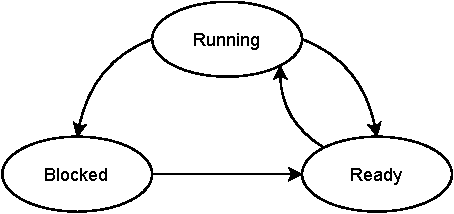
\includegraphics[width=0.5\linewidth]{basic}
	\end{center}
	
	A process cycles between each state multiple times within its lifetime. By
	default, a process is in the running state. If an I/O operation is
	required, the process enters the blocked state and waits until it is
	completed. After that, it proceeds to the ready state and waits to be given
	CPU time again.
	
	A CPU time scheduling model that is based on these three transitions is
	known as \textit{non-preemptive} scheduling. In this scheme, once a process
	is given CPU time, it holds it until it encounters an I/O block or it
	terminates. A process which never blocks or terminates may stall the
	execution of other processes indefinitely.
	
	However, a fourth transition is possible -- a process may leave the running
	state and enter the ready state directly. This is the case in
	\textit{preemptive} scheduling schemes, where the OS intentionally
	interrupts the process to share CPU time across other processes. This kind
	of scheduling is used in modern interactive operating systems.
    
    \subsection{Scheduling algorithms}
    
    Once a process loses CPU time, an algorithm chooses the next task to be
    scheduled. This choice may be made in several ways, ranging from simple to
    complex:
    
    \begin{enumerate}
        \item First come, first served -- processes registered earlier have
        priority over those registered later
        \item Round robin -- processes are scheduled in the order in which they
        were registered, looping over back to the first process
        \item Shortest job first -- the OS estimates the time a process may
        take to execute and picks the shortest one
        \item Shortest remaining time first -- a preemptive version of the
        above algorithm where a task may be interrupted in favor of another one
        with a shorter estimated execution time
    \end{enumerate}
    
    \section{Laboratory task}
    
    The lab task involved configuring the scheduling simulator to simulate
    $N~\in~\{2;5;10\}$ tasks, each requiring 2000 ms of CPU time and becoming
    I/O blocked in 500 ms intervals. The total time of the simulation was set
    to 10 seconds.
    
    \subsection{Two processes}
    
    \begin{verbatim}
Process #   CPU Time    IO Blocking CPU Completed   CPU Blocked
0           2000 (ms)   500 (ms)    2000 (ms)       3 times
1           2000 (ms)   500 (ms)    2000 (ms)       3 times

Process: 0 registered...  (2000 500 0    0)
Process: 0 I/O blocked... (2000 500 500 500)
Process: 1 registered...  (2000 500 0    0)
Process: 1 I/O blocked... (2000 500 500  500)
Process: 0 registered...  (2000 500 500  500)
Process: 0 I/O blocked... (2000 500 1000 1000)
Process: 1 registered...  (2000 500 500  500)
Process: 1 I/O blocked... (2000 500 1000 1000)
Process: 0 registered...  (2000 500 1000 1000)
Process: 0 I/O blocked... (2000 500 1500 1500)
Process: 1 registered...  (2000 500 1000 1000)
Process: 1 I/O blocked... (2000 500 1500 1500)
Process: 0 registered...  (2000 500 1500 1500)
Process: 0 completed...   (2000 500 2000 2000)
Process: 1 registered...  (2000 500 1500 1500)
Process: 1 completed...   (2000 500 2000 2000)
    \end{verbatim}
	
	This simple example illustrates the basic principles of non-preemptive
	scheduling. Once a process is assigned CPU time, it may do with it as it
	pleases until it encounters an I/O block or it terminates. As seen in the
	log, context switching only happens upon these two events.
	
	\subsection{Five processes}
	
	    \begin{verbatim}
Process #	CPU Time	IO Blocking	CPU Completed	CPU Blocked
0			2000 (ms)	500 (ms)	2000 (ms)		3 times
1			2000 (ms)	500 (ms)	2000 (ms)		3 times
2			2000 (ms)	500 (ms)	2000 (ms)		3 times
3			2000 (ms)	500 (ms)	2000 (ms)		3 times
4			2000 (ms)	500 (ms)	2000 (ms)		3 times

Process: 0 registered... (2000 500 0 0)
Process: 0 I/O blocked... (2000 500 500 500)
Process: 1 registered... (2000 500 0 0)
Process: 1 I/O blocked... (2000 500 500 500)
Process: 0 registered... (2000 500 500 500)
Process: 0 I/O blocked... (2000 500 1000 1000)
Process: 1 registered... (2000 500 500 500)
Process: 1 I/O blocked... (2000 500 1000 1000)
Process: 0 registered... (2000 500 1000 1000)
Process: 0 I/O blocked... (2000 500 1500 1500)
Process: 1 registered... (2000 500 1000 1000)
Process: 1 I/O blocked... (2000 500 1500 1500)
Process: 0 registered... (2000 500 1500 1500)
Process: 0 completed... (2000 500 2000 2000)
Process: 1 registered... (2000 500 1500 1500)
Process: 1 completed... (2000 500 2000 2000)
Process: 2 registered... (2000 500 0 0)
Process: 2 I/O blocked... (2000 500 500 500)
Process: 3 registered... (2000 500 0 0)
Process: 3 I/O blocked... (2000 500 500 500)
Process: 2 registered... (2000 500 500 500)
Process: 2 I/O blocked... (2000 500 1000 1000)
Process: 3 registered... (2000 500 500 500)
Process: 3 I/O blocked... (2000 500 1000 1000)
Process: 2 registered... (2000 500 1000 1000)
Process: 2 I/O blocked... (2000 500 1500 1500)
Process: 3 registered... (2000 500 1000 1000)
Process: 3 I/O blocked... (2000 500 1500 1500)
Process: 2 registered... (2000 500 1500 1500)
Process: 2 completed... (2000 500 2000 2000)
Process: 3 registered... (2000 500 1500 1500)
Process: 3 completed... (2000 500 2000 2000)
Process: 4 registered... (2000 500 0 0)
Process: 4 I/O blocked... (2000 500 500 500)
Process: 4 registered... (2000 500 500 500)
Process: 4 I/O blocked... (2000 500 1000 1000)
Process: 4 registered... (2000 500 1000 1000)
Process: 4 I/O blocked... (2000 500 1500 1500)
Process: 4 registered... (2000 500 1500 1500)
    \end{verbatim}
	
	This example serves to illustrate the ''first come, first served" algorithm
	used to choose which task is to be scheduled after the current one was
	blocked or terminated. As evident, processes which entered the queue earlier
	have priority over those that came later. Process 2 isn't allowed to run
	until after process 0 has terminated. Before that, processes 0 and 1 run
	alternatingly.
	
	\subsection{Ten processes}
	
	\begin{verbatim}
Process #	CPU Time	IO Blocking	CPU Completed	CPU Blocked
0		2000 (ms)	500 (ms)	2000 (ms)	3 times
1		2000 (ms)	500 (ms)	2000 (ms)	3 times
2		2000 (ms)	500 (ms)	2000 (ms)	3 times
3		2000 (ms)	500 (ms)	2000 (ms)	3 times
4		2000 (ms)	500 (ms)	1000 (ms)	2 times
5		2000 (ms)	500 (ms)	1000 (ms)	1 times
6		2000 (ms)	500 (ms)	0 (ms)		0 times
7		2000 (ms)	500 (ms)	0 (ms)		0 times
8		2000 (ms)	500 (ms)	0 (ms)		0 times
9		2000 (ms)	500 (ms)	0 (ms)		0 times

Process: 0 registered... (2000 500 0 0)
Process: 0 I/O blocked... (2000 500 500 500)
Process: 1 registered... (2000 500 0 0)
Process: 1 I/O blocked... (2000 500 500 500)
Process: 0 registered... (2000 500 500 500)
Process: 0 I/O blocked... (2000 500 1000 1000)
Process: 1 registered... (2000 500 500 500)
Process: 1 I/O blocked... (2000 500 1000 1000)
Process: 0 registered... (2000 500 1000 1000)
Process: 0 I/O blocked... (2000 500 1500 1500)
Process: 1 registered... (2000 500 1000 1000)
Process: 1 I/O blocked... (2000 500 1500 1500)
Process: 0 registered... (2000 500 1500 1500)
Process: 0 completed... (2000 500 2000 2000)
Process: 1 registered... (2000 500 1500 1500)
Process: 1 completed... (2000 500 2000 2000)
Process: 2 registered... (2000 500 0 0)
Process: 2 I/O blocked... (2000 500 500 500)
Process: 3 registered... (2000 500 0 0)
Process: 3 I/O blocked... (2000 500 500 500)
Process: 2 registered... (2000 500 500 500)
Process: 2 I/O blocked... (2000 500 1000 1000)
Process: 3 registered... (2000 500 500 500)
Process: 3 I/O blocked... (2000 500 1000 1000)
Process: 2 registered... (2000 500 1000 1000)
Process: 2 I/O blocked... (2000 500 1500 1500)
Process: 3 registered... (2000 500 1000 1000)
Process: 3 I/O blocked... (2000 500 1500 1500)
Process: 2 registered... (2000 500 1500 1500)
Process: 2 completed... (2000 500 2000 2000)
Process: 3 registered... (2000 500 1500 1500)
Process: 3 completed... (2000 500 2000 2000)
Process: 4 registered... (2000 500 0 0)
Process: 4 I/O blocked... (2000 500 500 500)
Process: 5 registered... (2000 500 0 0)
Process: 5 I/O blocked... (2000 500 500 500)
Process: 4 registered... (2000 500 500 500)
Process: 4 I/O blocked... (2000 500 1000 1000)
Process: 5 registered... (2000 500 500 500)
    \end{verbatim}
	
	This example serves to illustrate the limitations of non-preemptive FIFO
	scheduling. If there isn't sufficient CPU time available in total to be
	divided among the processes, some processes may not receive any time at all.
	In this case, processes 0 through 3 got all the time they needed,
	processes 4 and 5 ran alternatingly until the simulation time ran out, and
	processes 6 through 9 never got to run at all.
    
\end{document}
